\chapter{Segulsvið}
% Intro to chapter, laws of force
Segulsvið eru kraftasvið sem eru náteng rafsviðum en hafa samt talsvert
frábrugðna hegðun í samanburði við rafsvið. Segulsvið myndast frá nokkrum gerðum
af málmum, þá nær innri uppbyging efnisins skapa náttúrulegt segulsvið útfrá
hreyfingu rafeinda.

Helsti munurinn á segulsviði og rafsviði er að segulsvið þurfa að flæða í
hringrás. Það leiðir til þess að efni sem er segulmagnað verður að mynda
segulpóla sem eru nefndir norður og suðurpólar. Síðan verkar krafturinn
sem hleðsla upplifir í segulsviði er hornréttur á hreyfiátt hleðslu og
stefnu segulsviðs.

Helsta einingin sem er notuð er Tesla eða $\si{\tesla}$. 
\section{Lögmál Lorentz}
% Examples of size, direction
\marginpar{
	Lorentz er ekki talinn hafa fundið Lögmál Lorentz en hann var sá fyrsti til
	finna skýra stærðfræðilega lýsingu á eiginleikum lögmálsins.
	}
Krafturinn sem hleðsla upplifir er gefinn við krossfeldið á milli hreyfistefnu
og segulsviðs, þá er nauðsynlegt að beita vigrum til að finna kraftstefnu.
Þá eru venslin sem mynda kraftinn gefinn við
\begin{align}
	\vec{\uforce} 
		&= \uchargeq \left( \vec{\uspeed} 
			\times \vec{\umfieldb}  \right)
\end{align}
það er ekki augljóst hvaða afleiðingar þetta hefur fyrir kraftinn sem verkar
á hleðsluna. Þá þarf að vinna úr dæmum með krossfeldum, sem geta verið fremur
ruglingsleg. Krafturinn, hraðinn og segulsviðið er þá gefið við
\begin{align*}
	\vec{\uforce} &= 
		\left( 
		\begin{array}{c} 
			\uforce_\ulengthx \\
			\uforce_\ulengthy \\
			\uforce_\ulengthz \\
		\end{array} 
		\right) \\
	\vec{\uspeed} &= 
		\left( 
		\begin{array}{c} 
			\uspeed_\ulengthx \\
			\uspeed_\ulengthy \\
			\uspeed_\ulengthz \\
		\end{array} 
		\right) \\
	\vec{\umfieldb} &= 
		\left( 
		\begin{array}{c} 
			\umfieldb_\ulengthx \\
			\umfieldb_\ulengthy \\
			\umfieldb_\ulengthz \\
		\end{array} 
		\right) \\
\end{align*}
þar sem $\uforce_\ulengthx$ táknar stærðkraftsins meðfram x-ás. Dæmi teikningu
á slíkum vigrum er 
\begin{center}
	% Need to figure out howto rotate the view
	% \tdplotsetmaincoords{60}{110}
	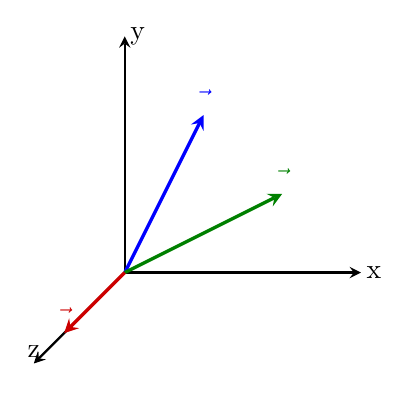
\begin{tikzpicture}[
		scale=1.0,
		%Option for nice arrows
		>=stealth, %
		inner sep=0pt, outer sep=2pt,%
		axis/.style={thick,->},
		wave/.style={very thick,color=#1,smooth, ->},
		polaroid/.style={fill=black!60!white, opacity=0.3},
	]
		% Colors
		\colorlet{darkgreen}{green!50!black}
		\colorlet{lightgreen}{green!80!black}
		\colorlet{darkred}{red!50!black}
		\colorlet{lightred}{red!80!black}

		% Frame
		\coordinate (O) at (0, 0, 0);
		\draw[axis] (O) -- +(3, 0,   0) node [right] {x};
		\draw[axis] (O) -- +(0,  3, 0) node [right] {y};
		\draw[axis] (O) -- +(0,  0,   3) node [above] {z};
		
		\draw[wave = blue] (O) -- +(1,  2,  0) 
			node [above] {$\vec{\uspeed}$};
		\draw[wave = darkgreen] (O) -- +(2,  1,  0) 
			node [above] {$\vec{\umfieldb}$};
		\draw[wave = lightred] (O) -- +(0,  0,  2) 
			node [above] {$\vec{\uforce}$};
	\end{tikzpicture}
\end{center}
þar sem krafturinn verkar einmitt hornrétt á tvo vigra. Þá leiðir til þess
að krafturinn er ekki samsíða hreyfi stefnunni. Dæmi um þetta væri segulsviðið
sem myndast umhverfis leiðara, það myndast hornrétt á hreyfistefnu rafeindanna
í leiðaranum. Stærð kraftins er hægt að finna með
\begin{align*}
	\left| 
	\vec{\uforce} \right|
		&= \left| \uchargeq \left( \vec{\uspeed} 
			\times \vec{\umfieldb}  \right) \right| 
			\\
		&= \uchargeq \left|  \vec{\uspeed}  \right| \left| \vec{\umfieldb} \right| 
			\sin(\theta)
\end{align*}
þar sem $ v = \left|  \vec{\uspeed}  \right| $ er lengd hraðavigursins og
$B = \left| \vec{\umfieldb} \right|$ er lengd segulsviðsvigurs. Þá er $\theta$
hornið á milli vigrana $\vec{\uspeed}$ og $\vec{\umfieldb}$, hægt er að finna
hornið á milli þeirra með að leysa út $\cos(\theta) | \vec{\umfieldb} |
| \vec{\uspeed} | = \vec{\umfieldb} \cdot \vec{\uspeed}$.
\begin{formalexample}
	Rafeind ferðast í lárréttu plani, hornrétt á rafeinda í planinu er segulsvið.
	Hraði rafeindarinnar er $\SI{15e3}{\m\per\s}$ og styrkur segulsviðsins er
	$\SI{0.5e-4}{\tesla}$. Í vigurformi er það
	\begin{align*}
	\vec{\uspeed} &= 
		\left( 
		\begin{array}{c} 
			$\SI{15e3}{\m\per\s}$ \\
			$0$ \\
			$0$ \\
		\end{array} 
		\right)
	&
	\vec{\umfieldb} &= 
		\left( 
		\begin{array}{c} 
			0 \\
			$\SI{0.5e-4}{\tesla}$ \\
			0 \\
		\end{array} 
		\right)		
	\end{align*}
	\vspace{4 ex}
	Fyrst þarf að setja upp hnitakerfi, þá er valið að láta x-ásin vera samsíða
	hreyfistefnu rafeindarinnar, þar sem hornið á milli vigrana er $\theta = 
	\ang{90}$ vegna þess að þeir eru hornréttir á hvorn annan þá er
	stærð kraftsins gefin við
	\begin{align*}
		F 	&= 
			\uchargeq
			\left|  \vec{\uspeed}  \right| \left| \vec{\umfieldb} \right| 
				\sin(\theta) \\
			&= \uunitcharge \times \SI{15e3}{\m\per\s} \times \SI{0.5e-4}{\tesla} 
				\times \sin(\ang{90}) \\
			&= \SI{12.45e-20}{\N}
	\end{align*}
	sem er afar lítill kraftur sem verkar á rafeinda.
\end{formalexample}

\section{Straumur og segulsvið}
Þegar rafeindir eru á hreyfingu er það kallaður rafstraumur eða straumur,
hægt er að lýsa straumi með hraða og magni. Þeas. flæðið af rafeindum, eða
hleðslu er stjórnað af fjölda þeirra og magnið fyrir einhvern bút af leiðara á
tímaeiningu segir til um hraða þeirra.



\subsection{Beinn leiðari}

\subsection{Spóla}

\section{Lögmál Biot-Savart}

\section{Hleðsla í segulsviði}

\section{Segulflæði}


